\section{The Dependence of the Beam Coupling Impedance on the Kicker Components}

As part of the study to improve the beam screen it was decided to investigate systematically the effect of the various components of the kicker magnet on the resulting beam coupling impedance. This is divided into two sections, the study of the effect of the beam screen on the beam coupling impedance of the ferrite yoke, and subsequently a study of the effects of the dimensions of the beam screen and screen conductors on the beam coupling impedance.

\subsection{The Impedance of the MKI - Effects of the Inclusion of the Beam Screen}

To first judge the effectiveness of the concept of the beam screen as an impedance reduction technique we simulate the MKI by systematically adding components to the magnet to determine their effect on the beam coupling impedance. We consider the following configurations of the MKI:

\begin{enumerate}
\item{The c-core ferrite yoke}
\item{The c-core ferrite yoke with a ceramic tube in the aperture}
\item{As "2" above but with 24 screen conductors inserted into the ceramic tube, capactively coupled at one end}
\item{The internal magnet structure including the vacuum tank, HV and ground plates and the surrounding connections}
\end{enumerate}

These geometries are shown in Fig.~\ref{fig:mki-layout-buildup}, and the resulting impedance simulations for the real component shown in Fig.~\ref{fig:mki-buildup-impedance}. Several points can be seen; firstly that the inclusion of the beam screen with screen conductors very effectively screens the beam from the other components of the kicker magnet - including the ceramic tube, the surrounding structures and the ferrite yoke itself. This indicates that for a beam screen in which the ceramic tube holds a large number of screen conductors, the beam is effectively screened from the surrounding structure up to a frequency characterised by the seperation of the screen conductors. This has benefits for the impedance simulations as it is valid to use a reduced simulation model considering just the capacitively coupled end provided we can assume the ferrite is well screened (i.e. we have 24 screen conductors in place). And lastly that the use of the ceramic tube contributes significantly to the imaginary component of the longitudinal impedance of the complete magnet (evidenced by the linear increase of the imaginary impedance, in cases 3 and 4 in the simulation results, with frequency due to the inductive component of the impedance) even with the presence of screen conductors.
 
\begin{figure}
\subfigure[]{
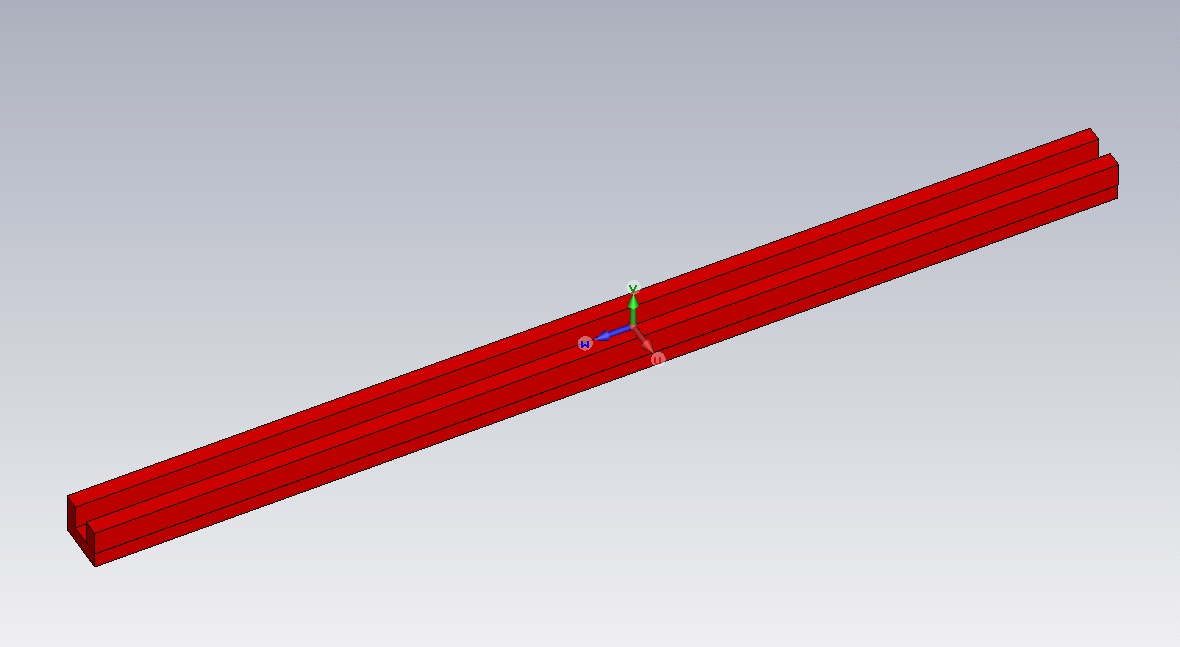
\includegraphics[width=0.45\textwidth]{LHC_MKI/figures/mki-buildup-ferrite.png}
\label{fig:mki-buildup-ferrite}
}
\subfigure[]{
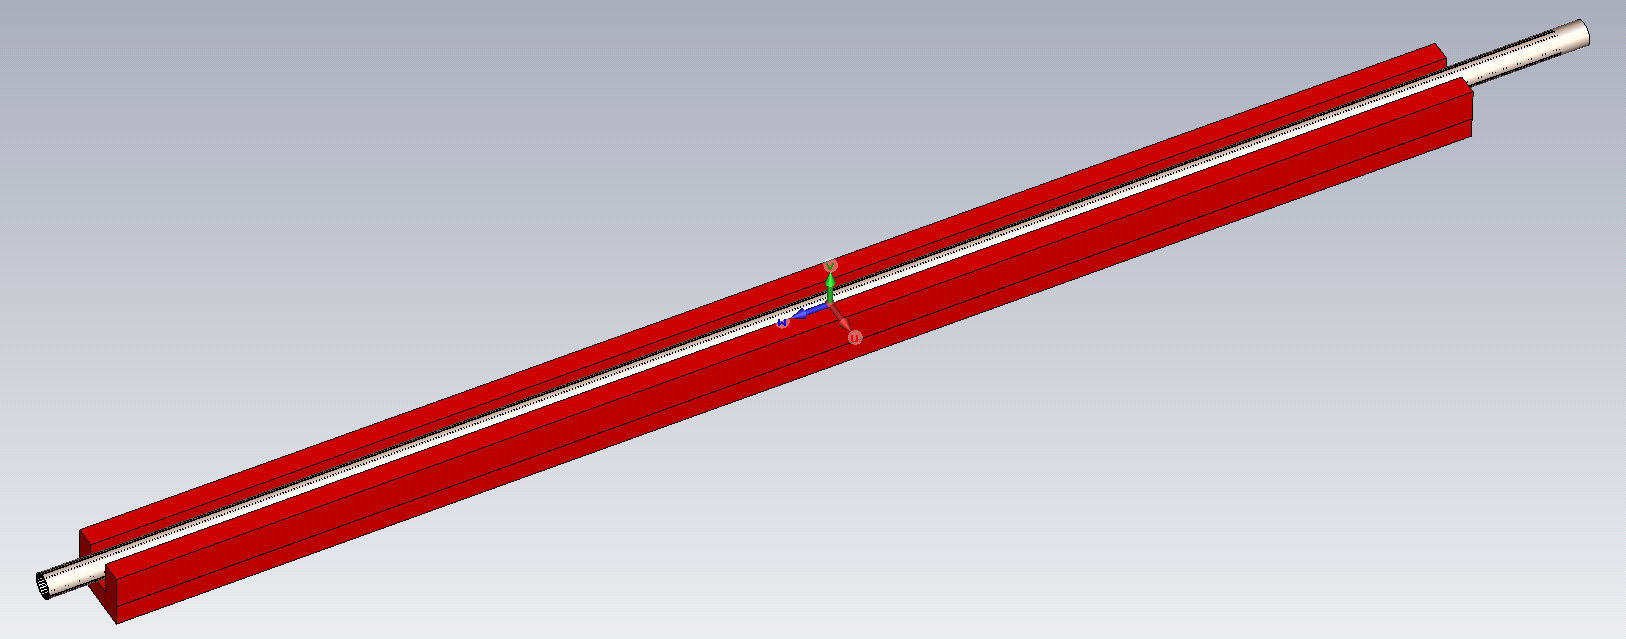
\includegraphics[width=0.45\textwidth]{LHC_MKI/figures/mki-buildup-ferrite-ceramic.png}
\label{fig:mki-buildup-ferrite-ceramic}
}
\subfigure[]{
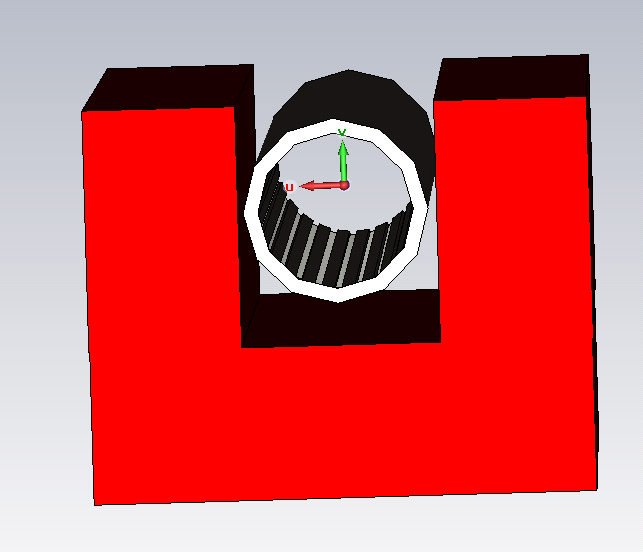
\includegraphics[width=0.45\textwidth]{LHC_MKI/figures/mki-buildup-ferrite-ceramic-cond.png}
\label{fig:mki-buildup-ferrite-ceramic-cond}
}
\subfigure[]{
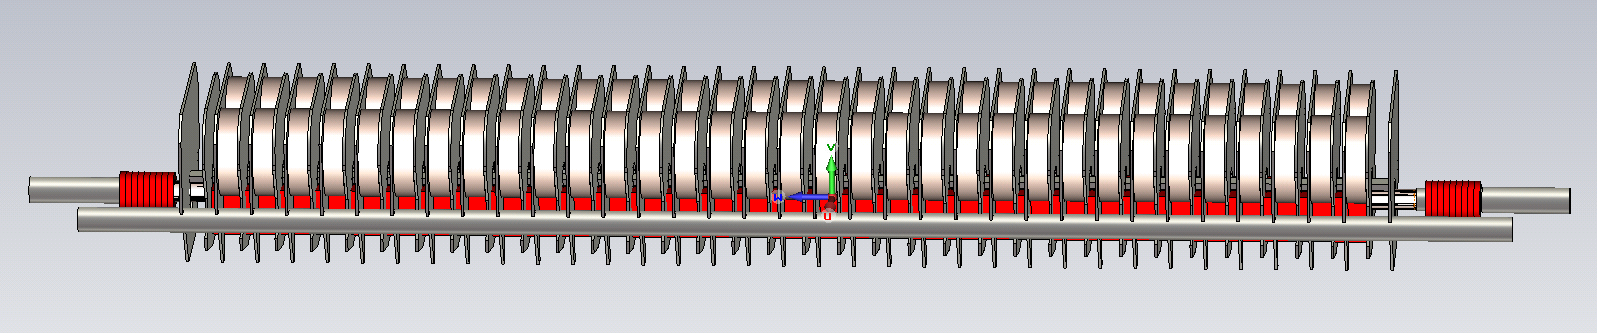
\includegraphics[width=0.45\textwidth]{LHC_MKI/figures/mki-buildup-ferrite-ceramic-cond-full.png}
\label{fig:mki-buildup-ferrite-ceramic-cond-full}
}
\caption{The geometries simulated for the various components in the LHC-MKI. These are c-core ferrite only \ref{fig:mki-buildup-ferrite}, c-core ferrite and the ceramic tube \ref{fig:mki-buildup-ferrite-ceramic}, c-core ferrite with the ceramic tube containing 24 screen conductors \ref{fig:mki-buildup-ferrite-ceramic-cond} and finally the complete MKI magnet (without vacuum tank for clarity) \ref{fig:mki-buildup-ferrite-ceramic-cond-full}.}
\label{fig:mki-layout-buildup}
\end{figure}

\begin{figure}
\subfigure[]{
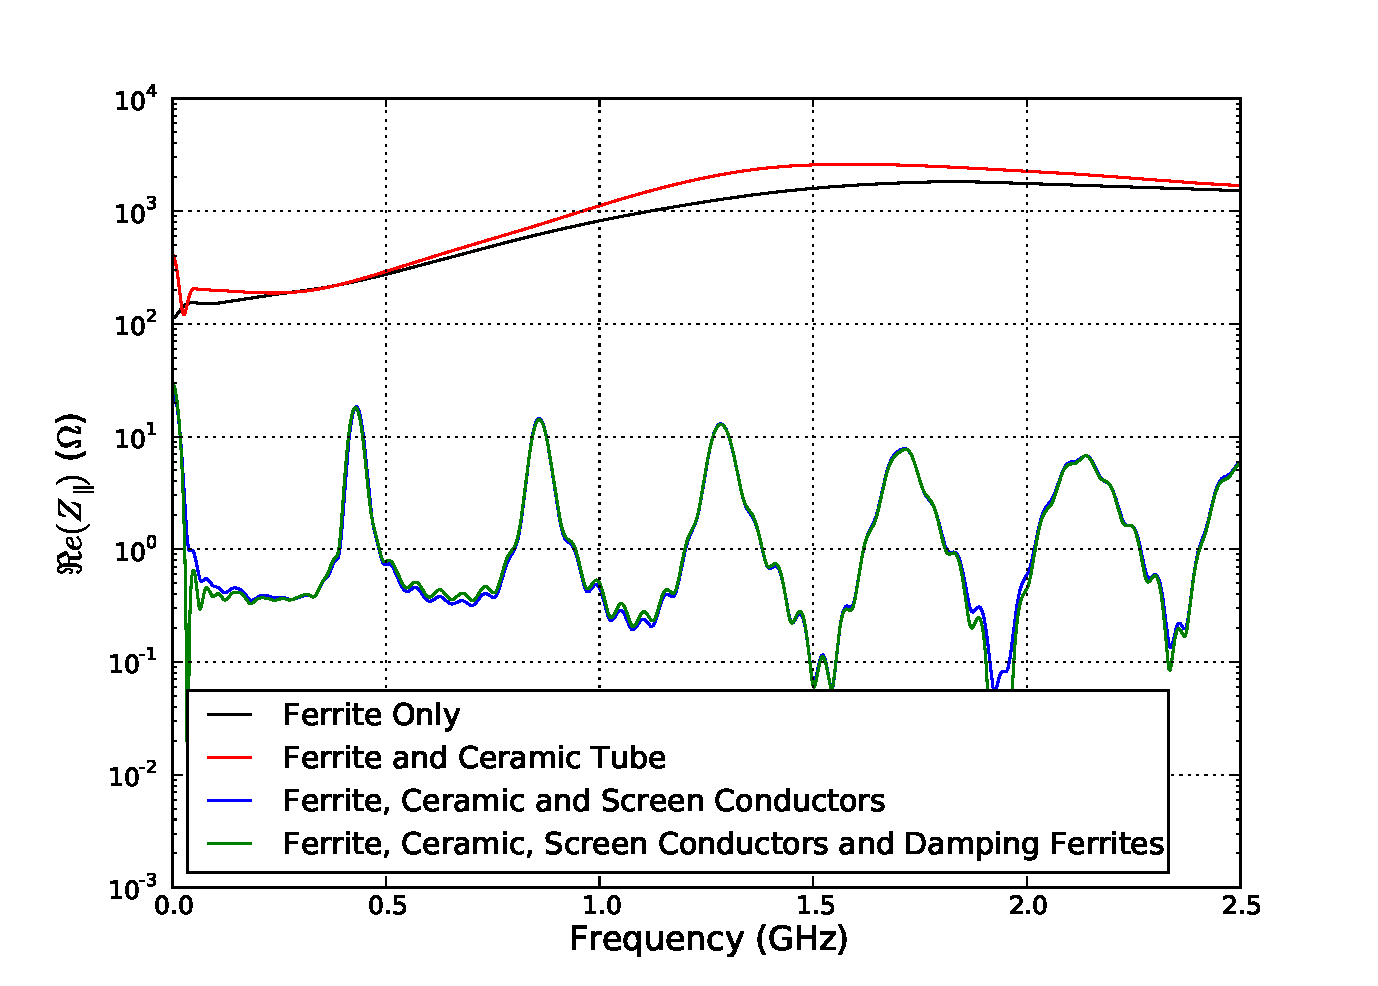
\includegraphics[width=0.5\textwidth]{LHC_MKI/figures/mki-build-up-real-imp.pdf}
\label{fig:mki-buildup-real-imp}
}
\subfigure[]{
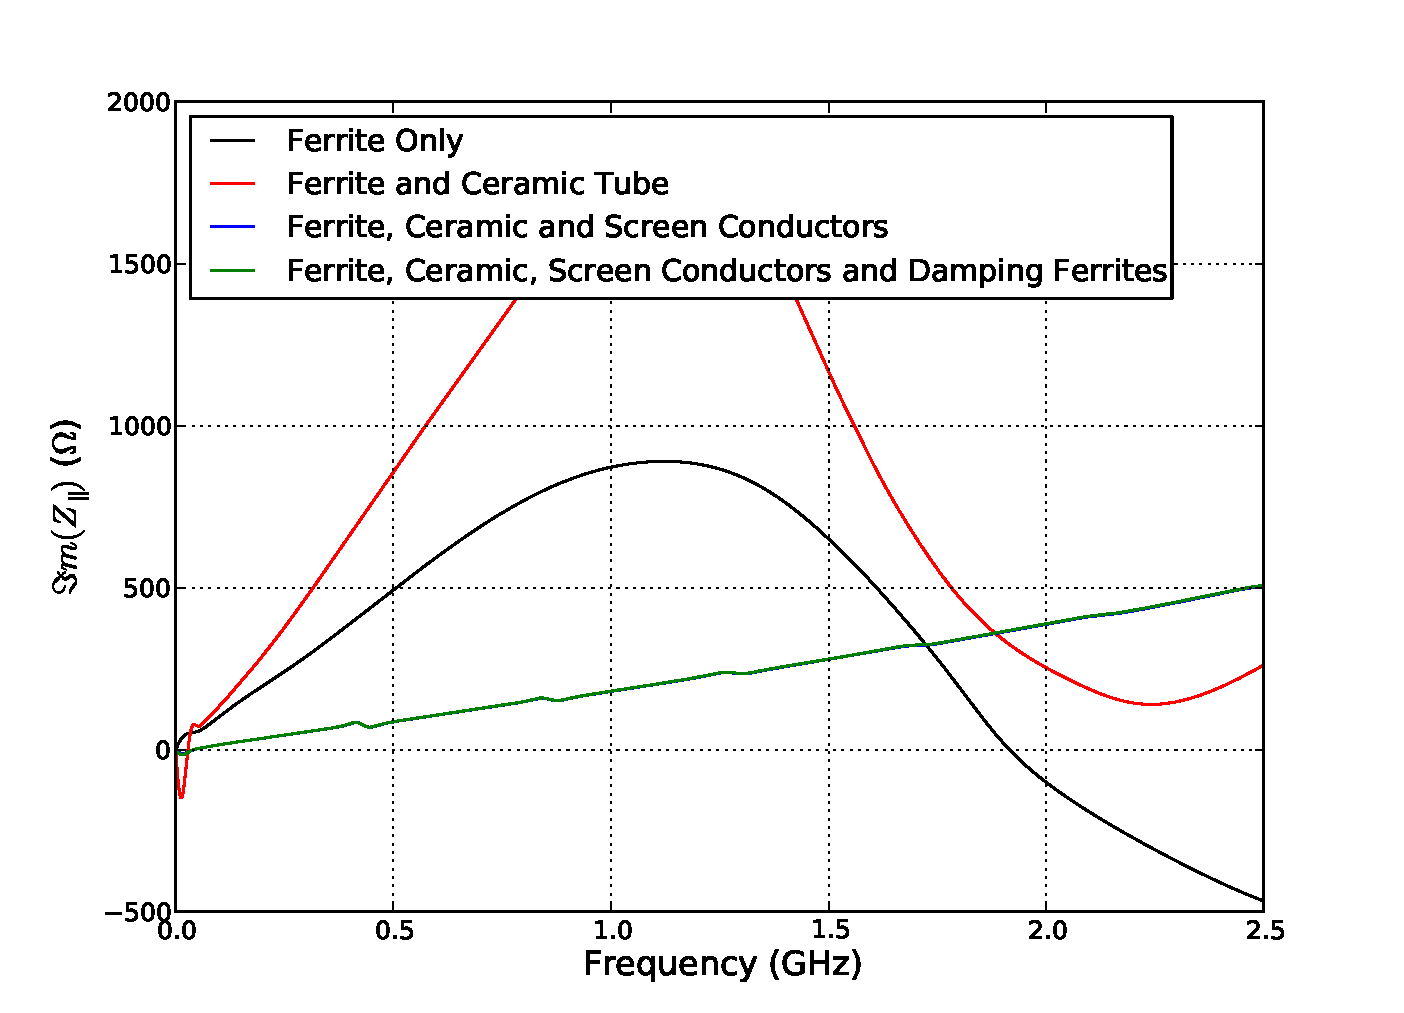
\includegraphics[width=0.5\textwidth]{LHC_MKI/figures/mki-build-up-imag-imp.pdf}
\label{fig:mki-buildup-imag-imp}
}
\caption{The \ref{fig:mki-buildup-real-imp} real component and the \ref{fig:mki-buildup-imag-imp} imaginary components of the LHC MKI kicker magnet impedances for different components in the magnet.}
\label{fig:mki-buildup-impedance}
\end{figure}


Concerning the role of the beam screen layout there are two areas to examine - the effect of different quantities of screening of the beam by having more or less screen conductors (in this case removing those directed towards the HV busbar due to concerns of electrical breakdown) and of the effect of different lengths of the screen conductors at the capacitively coupled end of the beam screen.

\subsection{How Screening Changes with the Number of Screen Conductors}

For the changes in the number of screen conductors two variations are carried out - The first is to examine the case of removing several screen conductors in the beam screen towards the HV busbar (shown in Fig.~\ref{fig:mki-take-away-cond-together}). This direction is chosen as these screen conductors experience the highest induced voltage during the pulsing of the kicker magnet, and additionally it was initially thought that on this side the HV busbar would provide some screening of the beam from the ferrite yoke. The second variation is to remove a selection of screen conductors towards the HV busbar (shown in Fig.~\ref{fig:mki-take-away-cond-alt}), in this case to examine whether it is possible to acquire some shielding through using some screen conductors and benefitting from removing some screen conductors to further reduce the rate of electrical breakdown.

\begin{figure}
\subfigure[]{
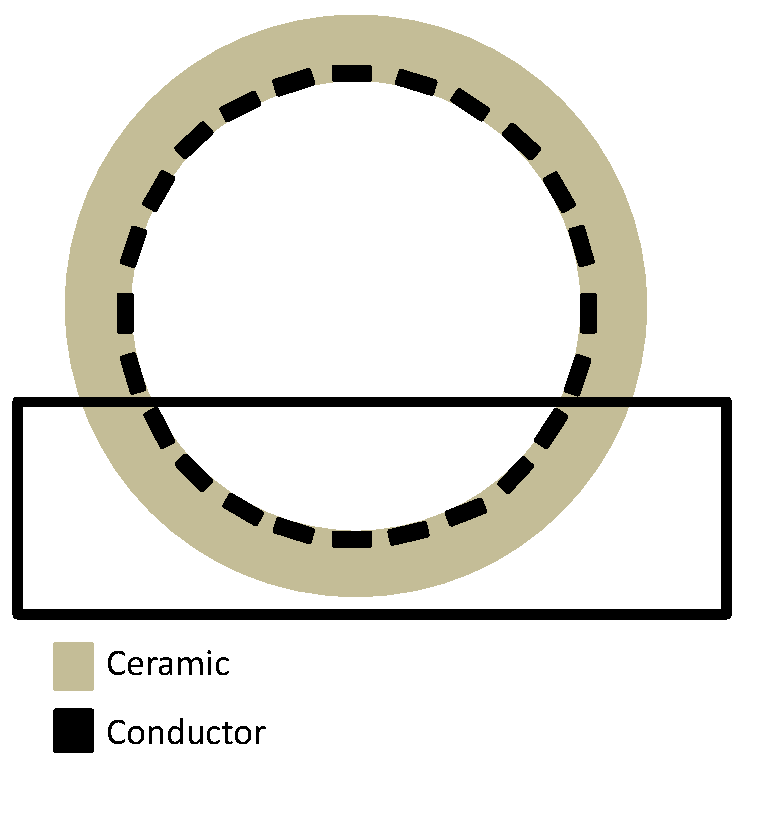
\includegraphics[width=0.3\textwidth]{LHC_MKI/figures/15-screen-cond.pdf}
\label{fig:15-cond-together}
}
\subfigure[]{
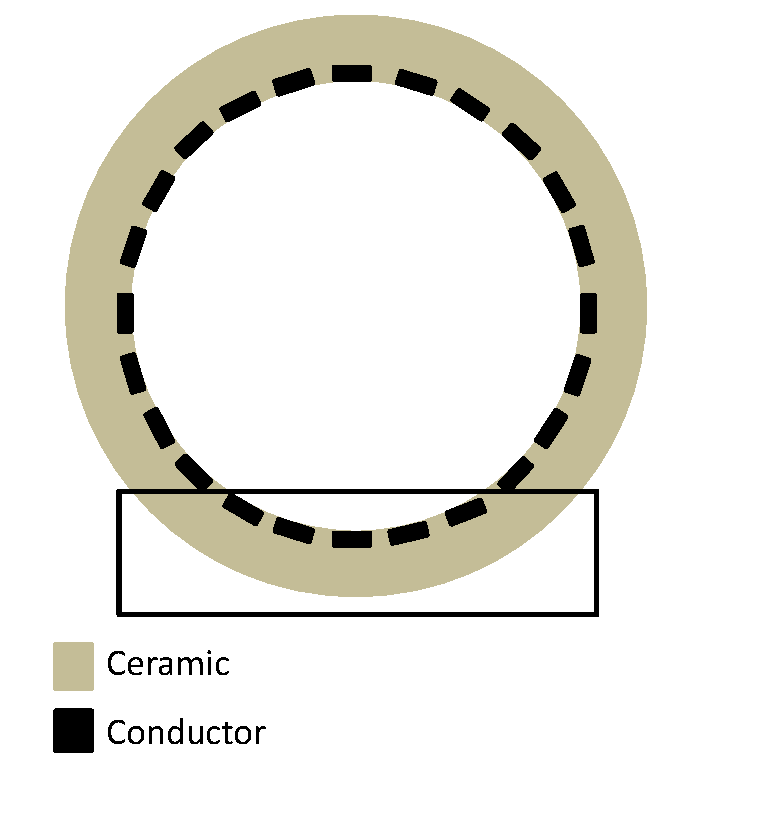
\includegraphics[width=0.3\textwidth]{LHC_MKI/figures/19-screen-cond.pdf}
\label{fig:19-cond-together}
}
\subfigure[]{
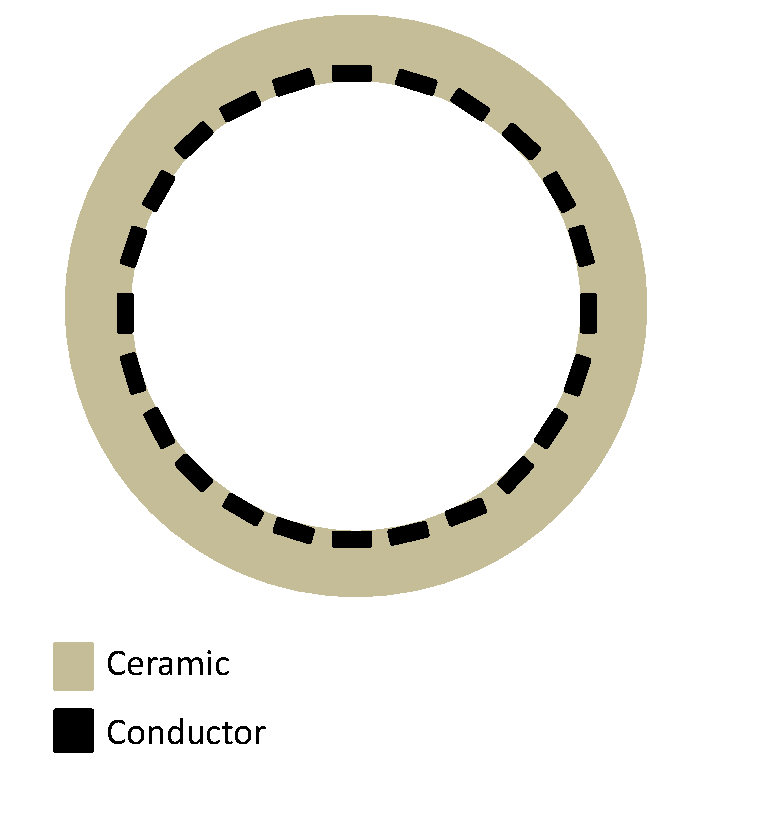
\includegraphics[width=0.3\textwidth]{LHC_MKI/figures/24-screen-cond.pdf}
\label{fig:24-cond-together}
}
\caption{Beam screens with different numbers of screen conductors removed from the design quantity of 24. Models of 15 \ref {fig:15-cond-together}, 19 \ref{fig:19-cond-together} and 24 \ref{fig:24-cond-together} screen conductors are considered for the impedance simulations. Conductors surrounded by the boxes are removed in this case.}
\label{fig:mki-take-away-cond-together}
\end{figure}

\begin{figure}
\subfigure[]{
\label{fig:17-cond-alt}
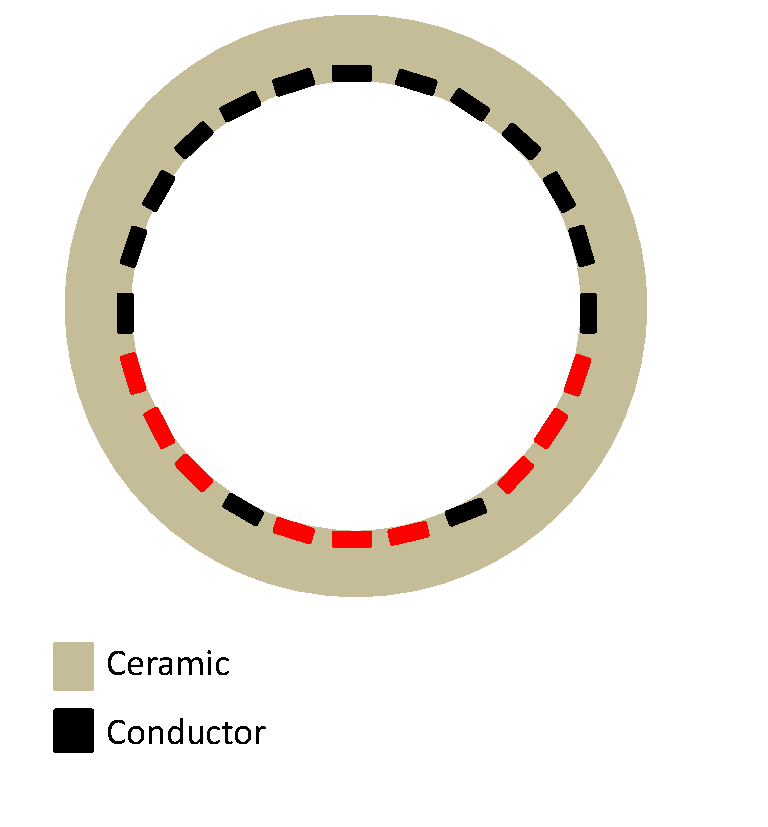
\includegraphics[width=0.45\textwidth]{LHC_MKI/figures/17-cond-alt.pdf}
}
\subfigure[]{
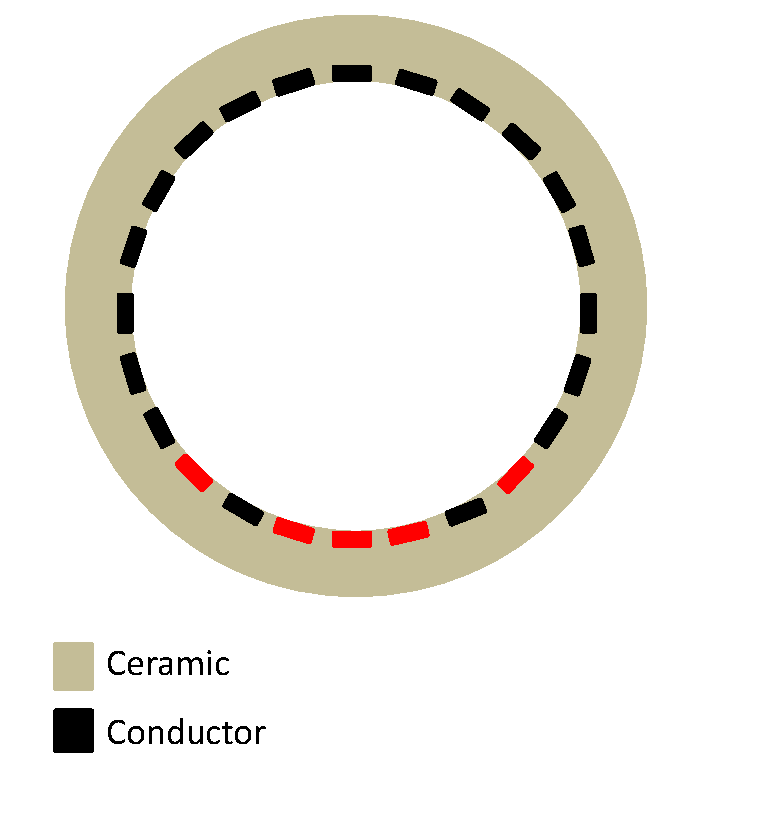
\includegraphics[width=0.45\textwidth]{LHC_MKI/figures/19-cond-alt.pdf}
\label{fig:19-cond-alt}
}
\subfigure[]{
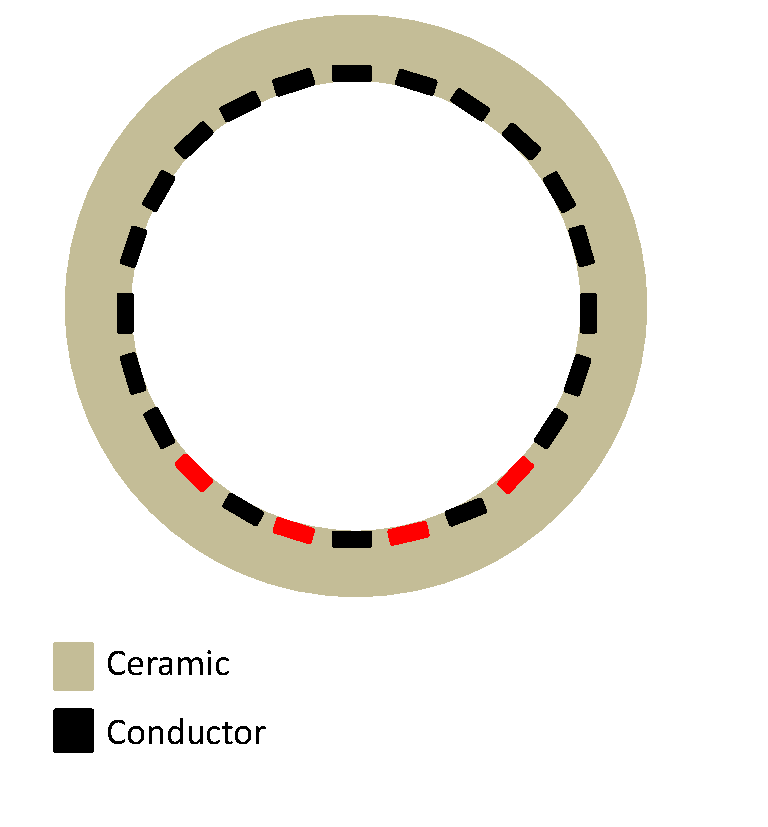
\includegraphics[width=0.45\textwidth]{LHC_MKI/figures/20-cond-alt.pdf}
\label{fig:20-cond-alt}
}
\subfigure[]{
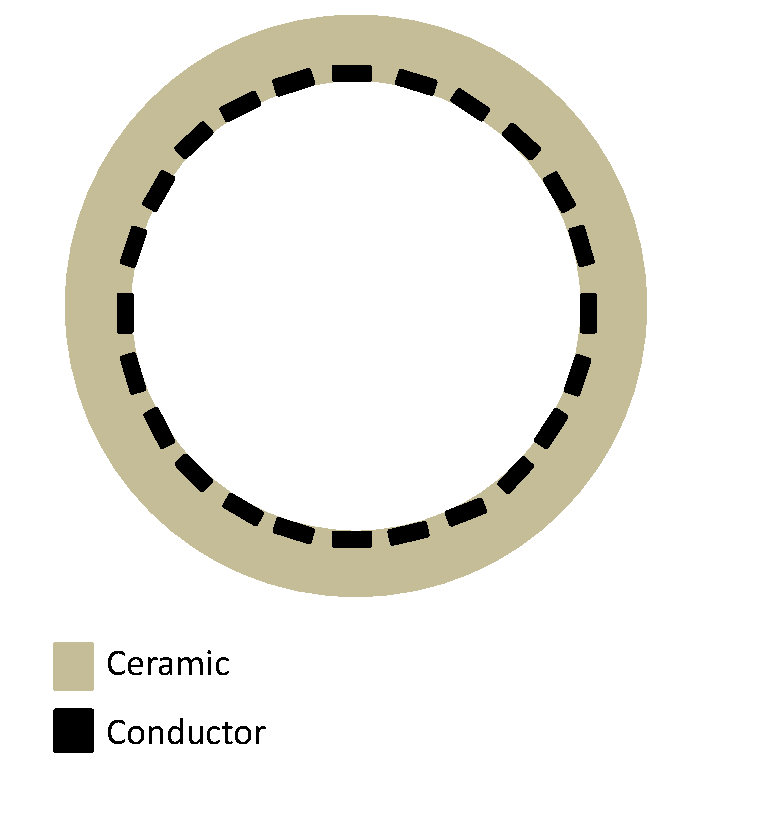
\includegraphics[width=0.45\textwidth]{LHC_MKI/figures/24-cond-alt.pdf}
\label{fig:24-cond-alt}
}
\caption{Beam screens with different numbers of screen conductors removed from the design quantity of 24. Models of 17 \ref {fig:17-cond-alt}, 19 \ref{fig:19-cond-alt}, 20 \ref{fig:20-cond-alt} and 24 \ref{fig:24-cond-alt} screen conductors are considered for the impedance simulations. Conductors that are coloured red are the removed in each case.}
\label{fig:mki-take-away-cond-alt}
\end{figure}

\begin{figure}
\subfigure[]{
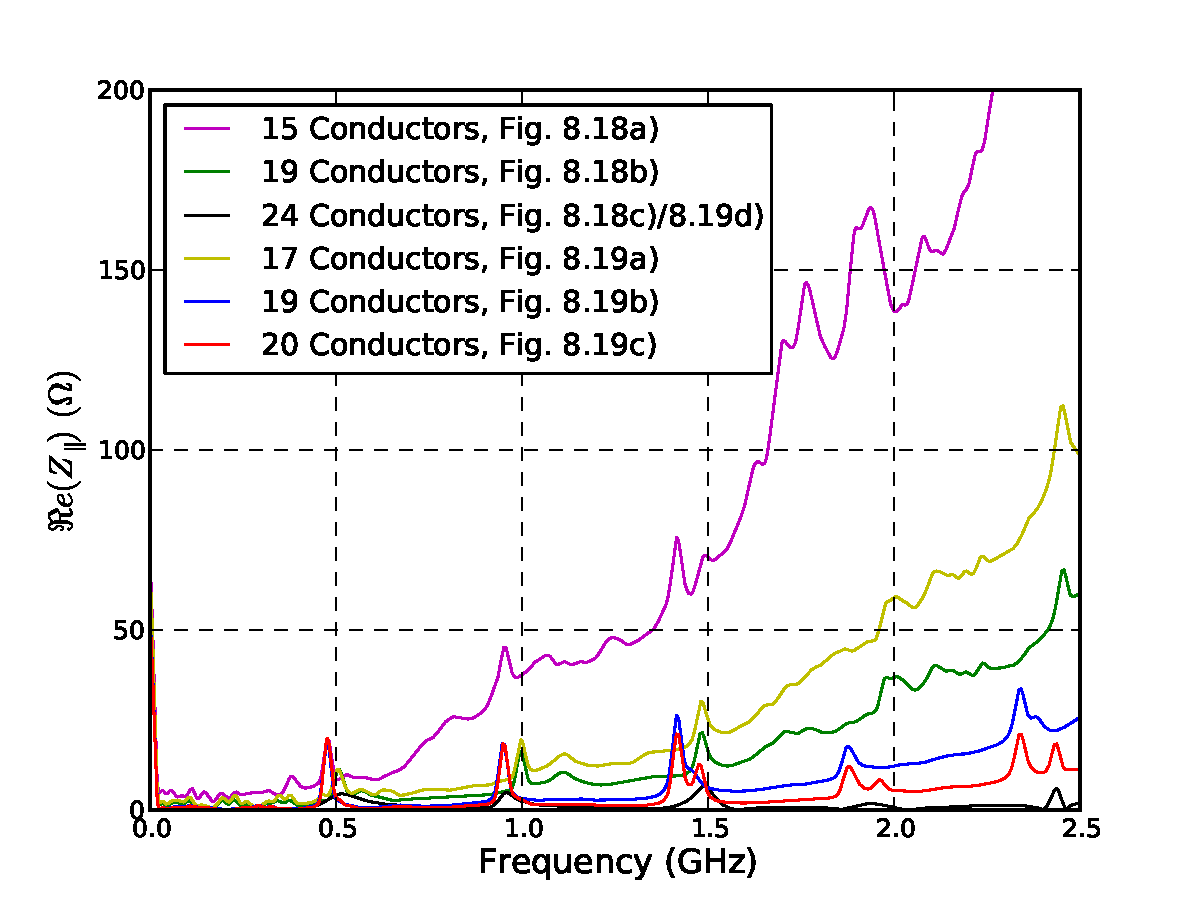
\includegraphics[width=0.5\textwidth]{LHC_MKI/figures/mki-no-screen-conductors-real-impedance.pdf}
\label{fig:remove-cond-real-imp}
}
\subfigure[]{
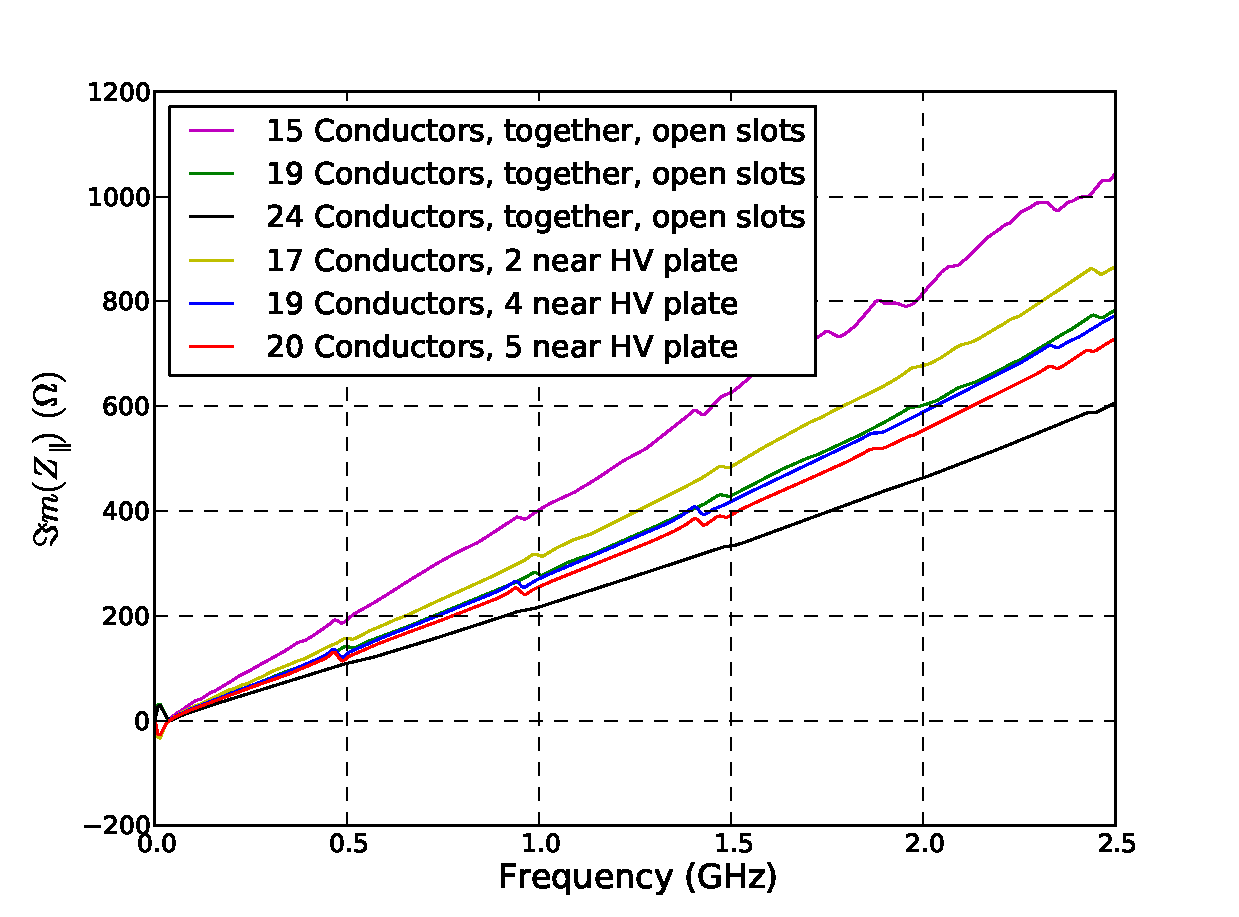
\includegraphics[width=0.5\textwidth]{LHC_MKI/figures/mki-no-screen-conductors-imag-impedance.pdf}
\label{fig:remove-cond-imag-imp}
}
\caption{The longitudinal impedance of the MKIs with different numbers of screen conductors included in the beam screen. Shown is the real component \ref{fig:remove-cond-real-imp} and the imaginary component \ref{fig:remove-cond-imag-imp} of the longitudinal impedance.}
\label{fig:remove-cond-impedance}
\end{figure}

The longitudinal impedance for these configurations is shown in Fig.~\ref{fig:remove-cond-impedance}. It can be seen that for both components of the impedance that more screen conductors reduces the magnitude of the impedance at all frequencies - this can simply be understood as improving the screening of the ferrite yoke from the beam with additional screen conductors. This can particularly be seen in the increase of the number of screen conductors from 15 to 19 to 24 conductors in total - The screening is improved dramatically in each subsequent case. 

In addition it can be seen that it is preferable to distribute the screen conductors such that the maximum arc of the beam screen without screen conductors is minimised. This can clearly be seen by comparing the case of 19 screen conductors where all conductors are clustered together (as was done for the replacement MKI8d (Fig.~\ref{fig:19-cond-together}) and for 19 screen conductors, where only 3 are missing close to the HV busbar (Fig.~\ref{fig:19-cond-alt}). Again this advantage is bourne out in the power lost in the structure. This is however not beneficial without consideration of the induced electric field during kicker pulsing, as the induced voltage on a given screen conductor is still the same, and thus surface flashover along the ceramic tube to the external metallization is not changed by this layout. It can thus be seen that the beam screen design itself must be optimised with regards to the induced screen conductor voltage before more conductors can be added to the ceramic tube to improve screening.

\subsection{Dependence of the Impedance on the Beam Screen Dimensions}

It will now be shown that with 24 screen conductors placed in the ceramic tube that the resulting impedance is dominated by the dimensions of the ceramic tube, the screen conductors and the external metallisation at the capacitively coupled end of the beam screen. To investigate how changes to certain parameters (specifically the length of the overlap between the screen conductors and the external metallization and the thickness of the ceramic tube) a cut down model of the kicker magnet is used, considering just the capactively coupled end of the kicker magnet (shown in Fig.~\ref{fig:cut-down-mki-cap-end}). This is done to allow a larger mesh density in this important (from the electrical and impedance point of view) region of the kicker magnet. In models of the full kicker magnet the mesh density is severely limited due to the large mesh generated in the entire magnet volume which subsequently may make the mesh very limited in near beam areas (for example in the ceramic tube between the screen conductors and the external metallization. A comparison of the meshes is shown in Fig.~\ref{fig:mki-mesh-com-cst}). 

\begin{figure}
\begin{center}
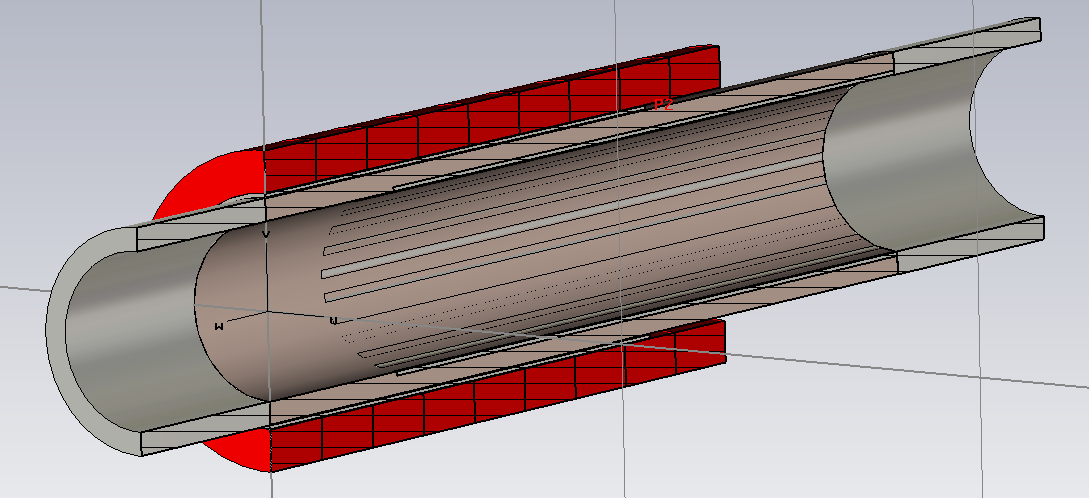
\includegraphics[width=0.75\textwidth]{LHC_MKI/figures/cutDownModel.png}
\end{center}
\caption{The cut down simulation model used for simulations of the MKI beam screen with 24 screen conductors.}
\label{fig:cut-down-mki-cap-end}
\end{figure}

\begin{figure}
\subfigure[]{
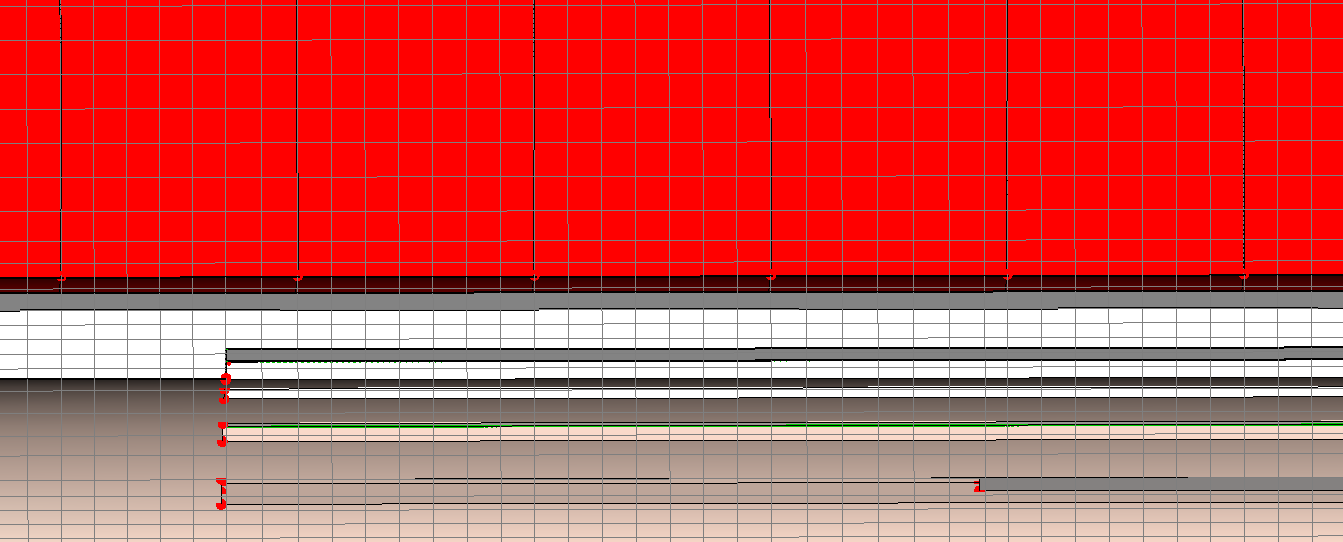
\includegraphics[width=0.45\textwidth]{LHC_MKI/figures/meshLarge.png}
\label{fig:mesh-full}
}
\subfigure[]{
\label{fig:mesh-cutdown}
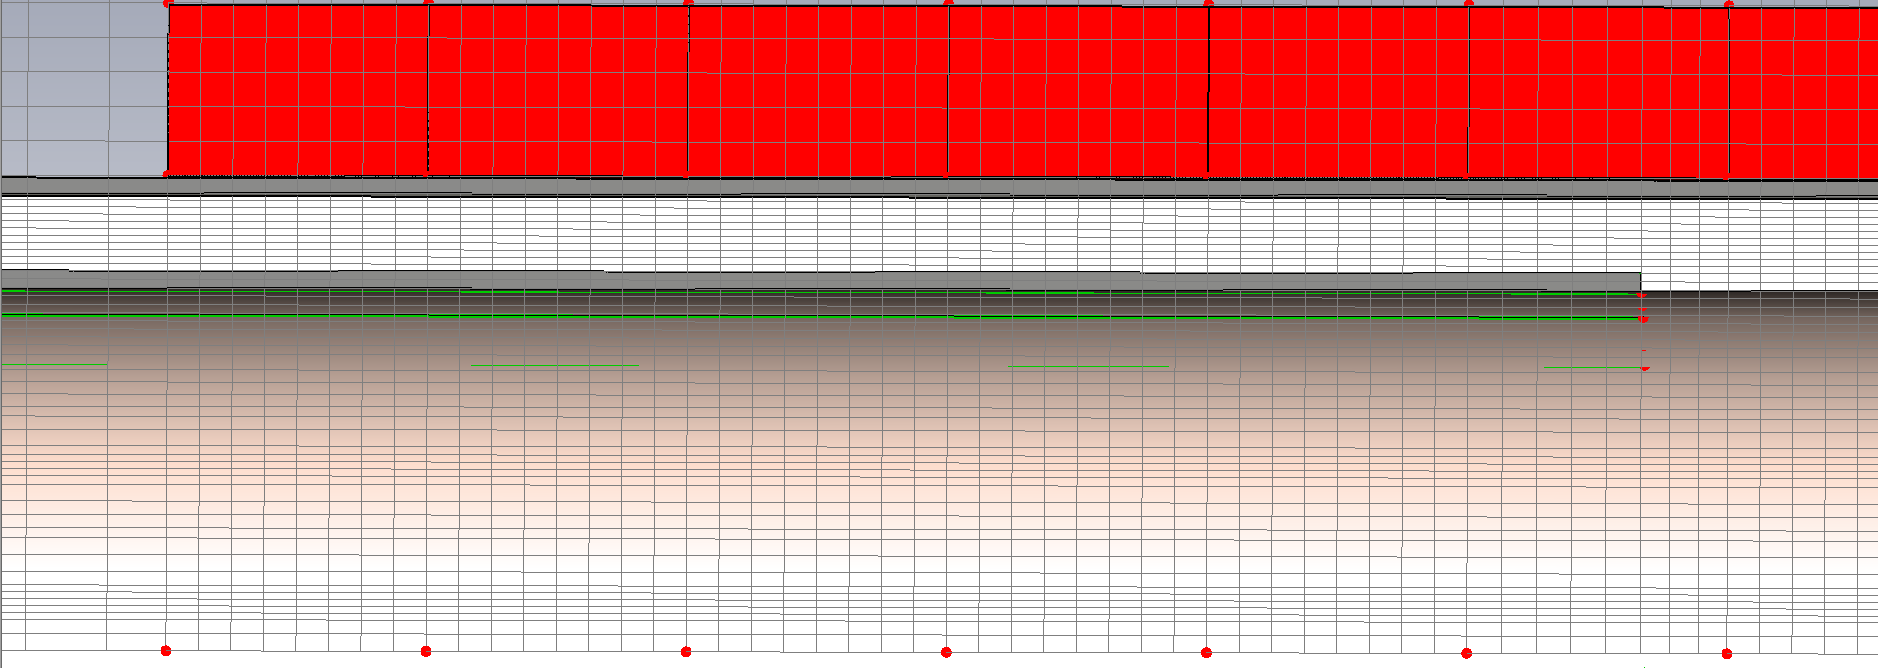
\includegraphics[width=0.45\textwidth]{LHC_MKI/figures/meshCutDown.png}
}
\caption{A comparison of the mesh that may be generated in CST Particle Studio using both the full model \ref{fig:mesh-full} and the cutdown model \ref{fig:mesh-cutdown}. Not the greatly increased mesh density in the important overlap region between the screen conductors and external metallization. The simulation time for the first is on the order a day, for the second 30 minutes.}
\label{fig:mki-mesh-com-cst}
\end{figure}

First we shall consider the effect the impedance for different lengths of overlap of the capacitively coupled sections. To do this we consider just the end section, and change the length of the external metallization to change the length of the overlap (the length of the screen conductors used is keep fixed to avoid changing any potential resonances due to the modelled length of the screen conductors acting as $\lambda /4$ resonators). Overlaps of between 0.08m and 0.12m at 0.01m intervals are simulated, and the results shown in Fig.~\ref{fig:overlap-imp}. It can be seen that each overlap has a distinct set of resonance frequencies. The source of these resonances can be seen to be the result of the overlap between the external metallization and the screen conductor acting as a $n \lambda /2$ resonator. End effects caused the effective length of the overlap to be extended to some degree, which fitting to the resonance frequencies has shown to be $\approx 9$mm for all lengths for a ceramic tube thickness of 7mm. This gives a resonant frequency $f_{res}$ of

\begin{equation}
f_{res} = \frac{nc}{\sqrt{\epsilon_{r}}2 \left( L_{overlap} + \delta_{fringe} \right)}
\label{eqn:imp-overlap-fres}
\end{equation}

where $n$ is an integer, $c$ is the speed of light $\epsilon_{r}$ is the relative permitivitty of the volume material ($\epsilon=10$ for the alumina beam screen), $L_{overlap}$ is the length of overlap and $\delta_{fringe}$ is the effective increase in length due to fringe fields. The resonant frequency calculated using Eqn.~\ref{eqn:imp-overlap-fres} is shown for the first resonances for all the effective lengths of overlap in Fig.~\ref{fig:overlap-imp-zoom}, and up to 2.5GHz for the case of the overlap being 100mm in Fig.~\ref{fig:imp-overlap-fres}. It can be seen that the predicted resonant frequencies match the simulated very well. Work is still under way as to how to determine the peak impedance of each resonance. In addition predictions for the power loss due to the impedances for different effective overlaps calculated assuming either a broadband heating scenario or assuming a beam harmonic at the resonant frequency as shown in Tab.~\ref{tab:heating-overlap}. It can be seen that changing the length of the overlap does not strongly correlate to the change in power loss assuming a broadband heating scenario. It can be seen that increasing the length of the effective overlap causes an increase in the power loss assuming a resonant heating scenario, but this correlation is not clear as there is much variance in the values.

\begin{figure}
\subfigure[]{
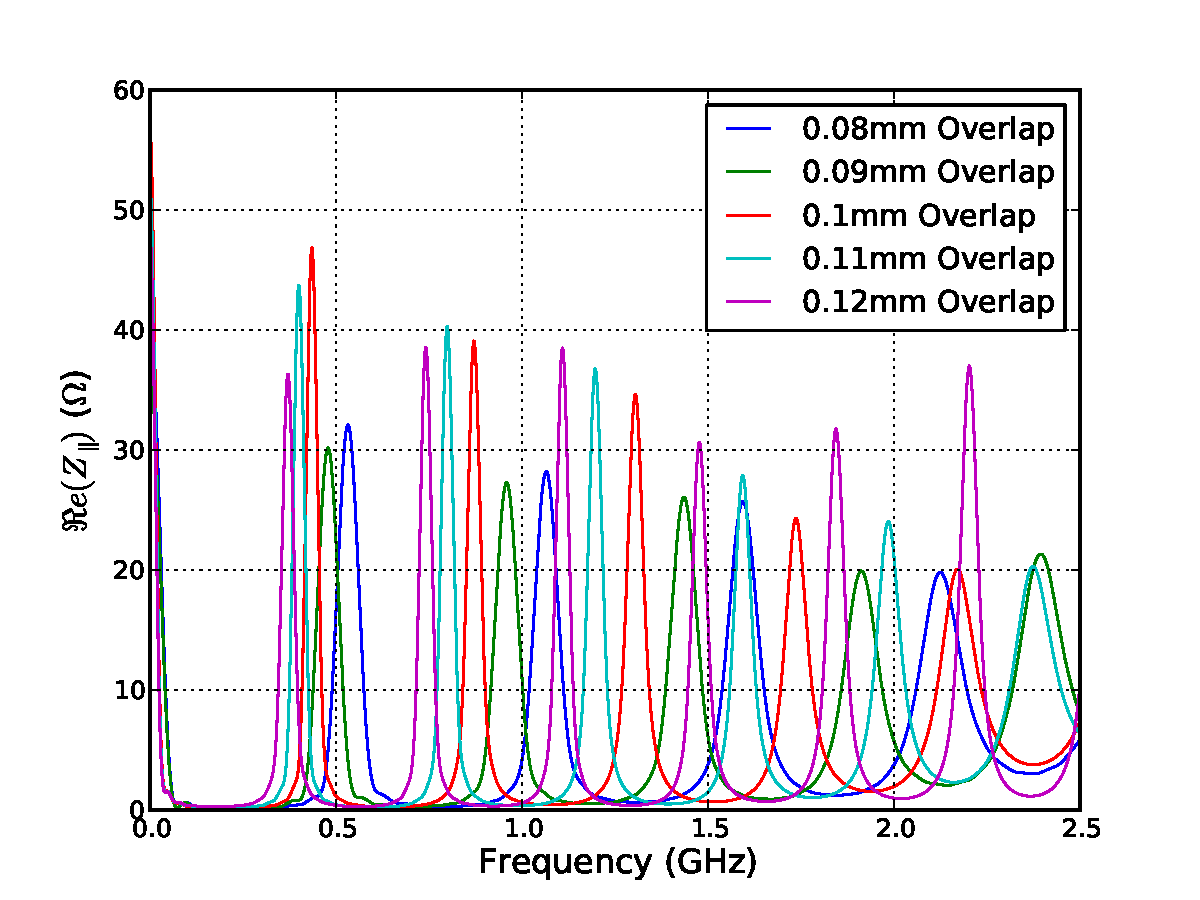
\includegraphics[width=0.5\textwidth]{LHC_MKI/figures/mki-overlap-len-real-imp.pdf}
\label{fig:overlap-imp}
}
\subfigure[]{
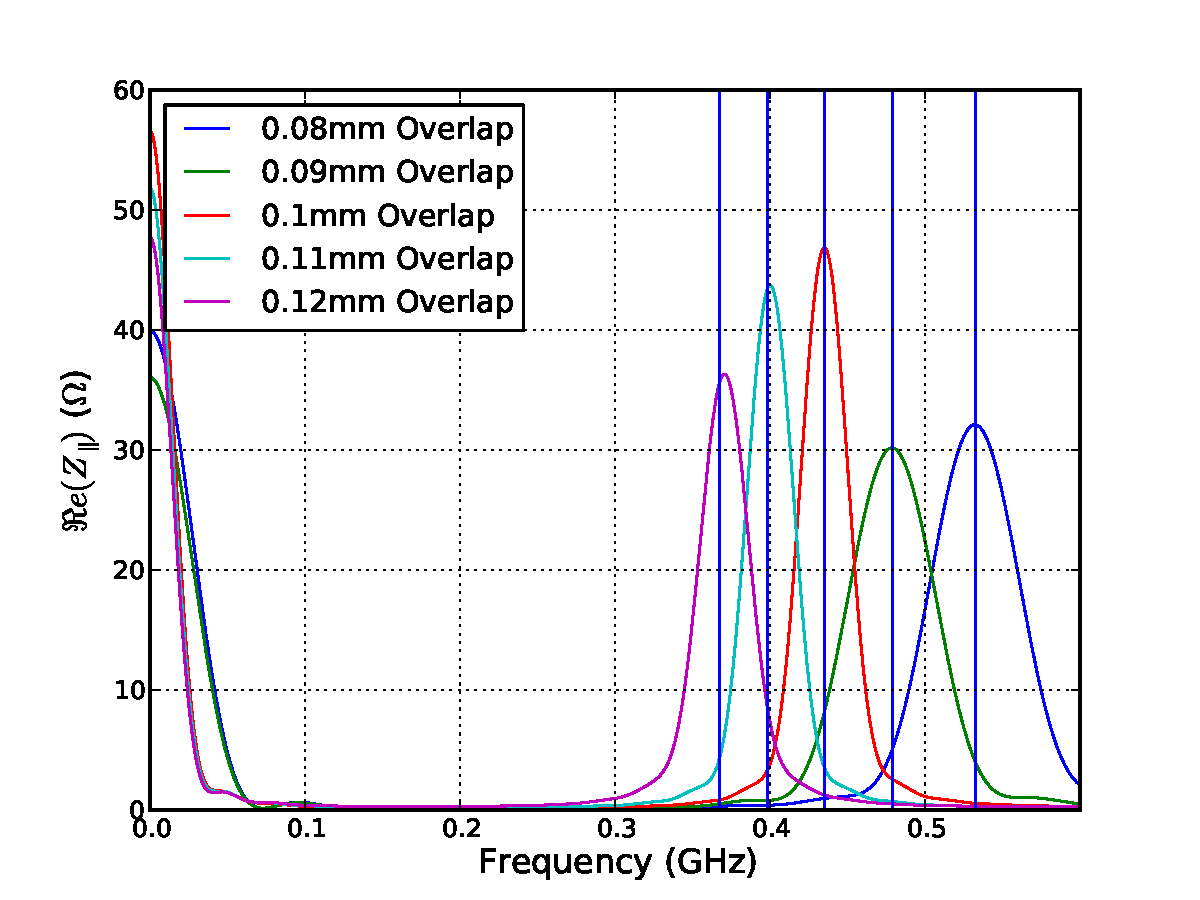
\includegraphics[width=0.5\textwidth]{LHC_MKI/figures/mki-overlap-len-real-imp-zoom.pdf}
\label{fig:overlap-imp-zoom}
}
\caption{\ref{fig:overlap-imp} The real component of the longitudinal beam coupling impedance for different lengths of the overlap, and \ref{fig:overlap-imp-zoom} a zoomed in plot of the first resonances of all the overlaps with the calculated resonance frequency for each based on the effective length. For each the thickness of the ceramic tube is 7mm.}
\label{fig:mki-overlap-imp-tot}
\end{figure}

\begin{figure}
\begin{center}
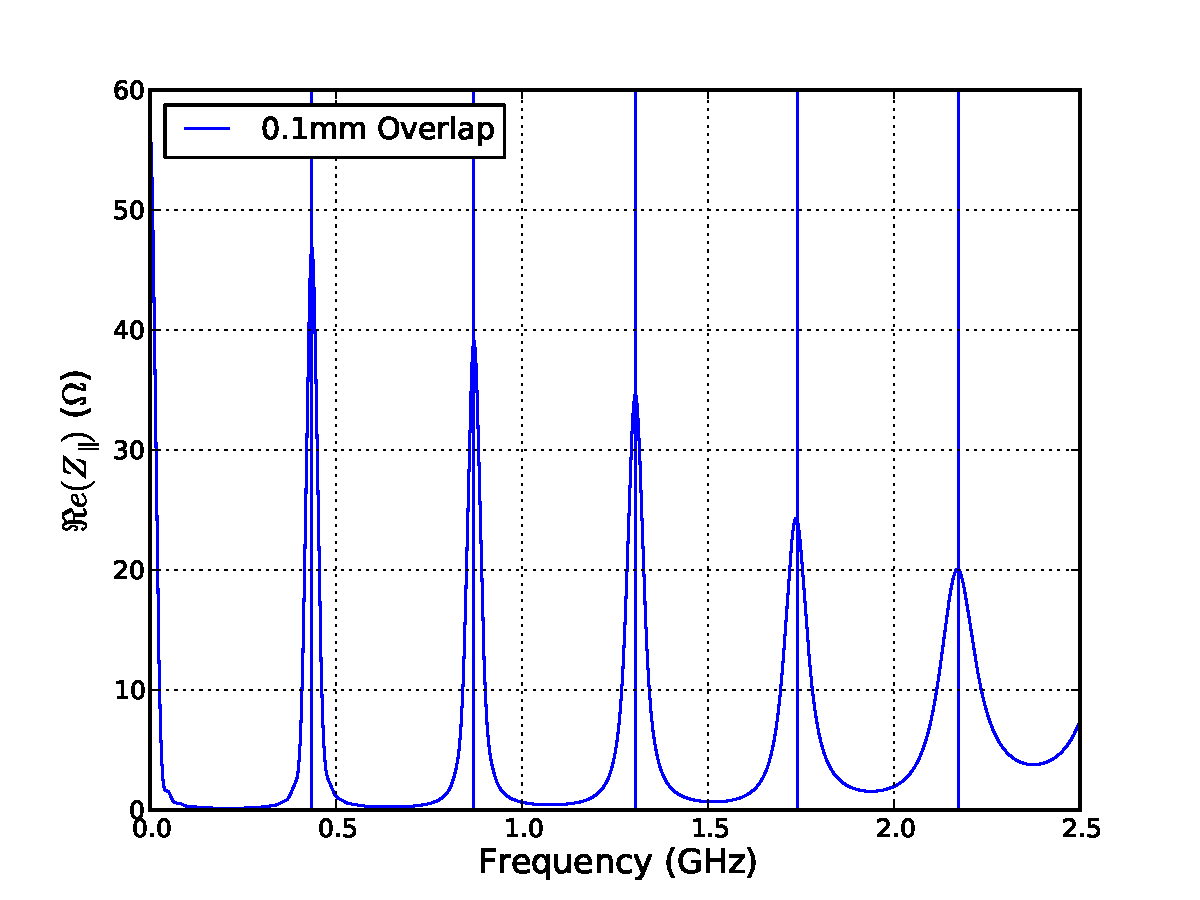
\includegraphics[width=0.6\textwidth]{LHC_MKI/figures/mki-overlap-fres-100mm.pdf}
\end{center}
\caption{The impedance of the beam screen with 24 screen conductors with an overlap $L_{overlap}=100mm$ and the predicted resonance frequencies from Eqn.~\ref{eqn:imp-overlap-fres} shown as vertical lines.}
\label{fig:imp-overlap-fres}
\end{figure}

\begin{table}
\caption{The beam induced heating calculated for a number of beam screen designs with 24 screen conductors with equal thickness of ceramic tube (thickness of 7mm) with different effective overlaps assuming 50ns bunch spacing LHC conditions (1380 bunches, $1.7\times 10^{11}$ppb with a bunch length of 1ns). It can be seen that the broadband heating component is relatively constant for the change in overlap, whilst the resonant component only significantly changes with a large increase in the effective overlap.}
\label{tab:overlap-heating}
\begin{center}
\begin{tabular}{c | c | c | c | c}
Overlap (mm)& \multicolumn{2}{c |}{LHC, 50ns, 1.7e11ppb} & \multicolumn{2}{|c}{LHC, 25ns, 1.15e11ppb} \\ \hline
 & BB (W) & Res(W) & BB (W) & Res (W) \\ \hline
80 & 38.5 & 6.9 & 30.0 & 13.0 \\ \hline
90 & 39.1 & 6.9 & 31.0 & 13.1 \\ \hline
100 & 35.3 & 12.1 & 28.8 & 23.0 \\ \hline
110 & 36.1 & 13.1 & 31.6 & 24.9 \\ \hline
120 & 36.7 & 12.7 & 28.9 & 24.1 \\ 
\end{tabular}
\end{center}
\end{table}

Secondly the influence of the thickness of the beam screen is considered. This is a concern as increasing this thickness has two effects - to change the value of the capcitance at the capacitively coupled end which effects the low frequency impedance, and the increase in the volume of the overlap region due to the increased thickness. The internal diameter of the ceramic tube is kept at 42mm, whilst external diameters of 50, 53 and 56mm are considered, giving tube thicknesses between 4 and 7mm. The resulting real component of the longitudinal impedances is shown in Fig.~\ref{fig:tube-thickness-imp}, where it can be seen that increasing the ceramic tube thickness has two effects - a slight lowering of the resonant frequency, but also a significant increase of the peak impedance of the resonance, by almost a factor 2 from a tube 4mm thick to a 7mm thick tube. The difference that the peak impedances make to the expected heating of the MKI can be seen in Tab.~\ref{tab:thickness-heating}, where it can be seen that the change in the power loss due to the increased thickness could be expected to be small assuming a broadband heating scenario, but increases significantly if we assume a beam harmonic falls upon the resonant frequency.

The small reduction in the resonant frequency as the thickness of the ceramic tube is increased is expected as the fringe fields will increase with greater thickness. The examination of the prediction shows that the increase in effective length, due to a non-zero thickness of the ceramic tube, is given (for $\epsilon_{r}$=10 for all frequencies) by an increase in effective length (in mm) of $\approx$ 0.0125$\times$thickness (in mm).

\begin{figure}
\begin{center}
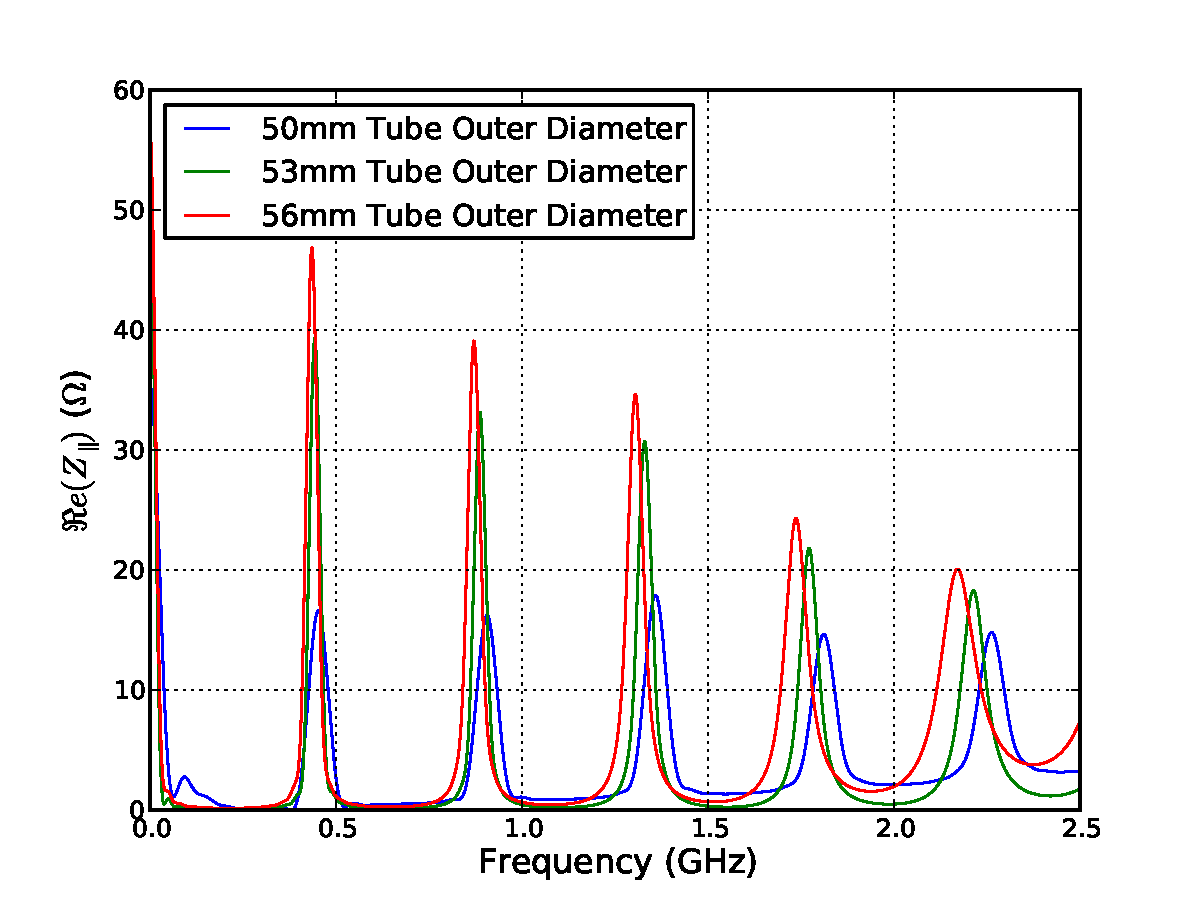
\includegraphics[width=0.5\textwidth]{LHC_MKI/figures/mki-tube-thickness-real.pdf}
\end{center}
\caption{The variance of the real beam coupling impedance with the tube thickness. External diameters of 50, 53 and 56mm correspond to tube thicknesses of 4, 5.5 and 7mm respectively. The physical overlap is 100mm in all cases.}
\label{fig:tube-thickness-imp}
\end{figure}

\begin{table}
\caption{The beam induced heating calculated for a number of beam screen designs with 24 screen conductors of equal length (overlap of 100mm) with different tube thicknesses assuming 50ns bunch spacing LHC conditions (1380 bunches, $1.7\times 10^{11}$ppb with a bunch length of 1ns). It can be seen that the change in broadband heating component does not strongly correlate with the change in tube thickness, whilst the resonant component can increase drastically due to the increasing peak impedance as a result of increasing the tube thickness.}
\label{tab:thickness-heating}
\begin{center}
\begin{tabular}{c | c | c }
Outer Tube Diameter/Tube Thickness (mm)  & $P_{loss, BB}$ & $P_{loss, Res}$ \\ \hline
50/4  & 30 & 4$ \\ \hline
53/5.5  & 26 & 10 \\ \hline
56/7  & 35 & 12 \\ 
\end{tabular}
\end{center}
\end{table}

